\subsubsection{Turbine} \label{sec:turb}
	We decided to use NREL's generalized 3.35MW reference turbine in all wind farms.
	It's attributes are open source, and it is designed as a baseline for onshore wind turbine specifications \cite{NREL335MW}.
	The specifics of the turbine needed for our simplified Gaussian wake model are located below:

	\begin{table}
		\begin{center}
			\caption{Attributes for NREL's 3.35MW onshore reference turbine}
			\label{tab:335MW}
			\begin{tabular}{@{}lrl@{}}
			\toprule
				Rotor Diameter & 130 & m \\ 
				Turbine Rating & 3.35 & MW \\ 
				Cut-In Wind Speed & 4 & m/s \\ 
				Rated Wind Speed & 9.8 & m/s \\ 
				Cut-Out Wind Speed & 25 & m/s \\
			\bottomrule
			\end{tabular}
		\end{center}
	\end{table}
		
	\noindent The power curve is defined as:   

	\begin{minipage}{0.53\textwidth}
		\begin{equation*}
			P(V) = 
			\begin{cases} 
				0 & V < V_{\textit{cut-in}} \\
				P_{\textit{rated}}\cdot\bigg(\frac{V-V_{\textit{cut-in}}}{V_{\textit{rated}}-V_{\textit{cut-in}}}\bigg)^3 & V_{\textit{cut-in}}\leq V < V_{\textit{rated}} \\
				P_{\textit{rated}} & V_{\textit{rated}} \leq V < V_{\textit{cut-out}} \\
				0 & V \geq V_{\textit{cut-out}}
			\end{cases}
		\label{eq:power}
		\end{equation*}
	\end{minipage}\quad
	\begin{minipage}{0.53\textwidth}
		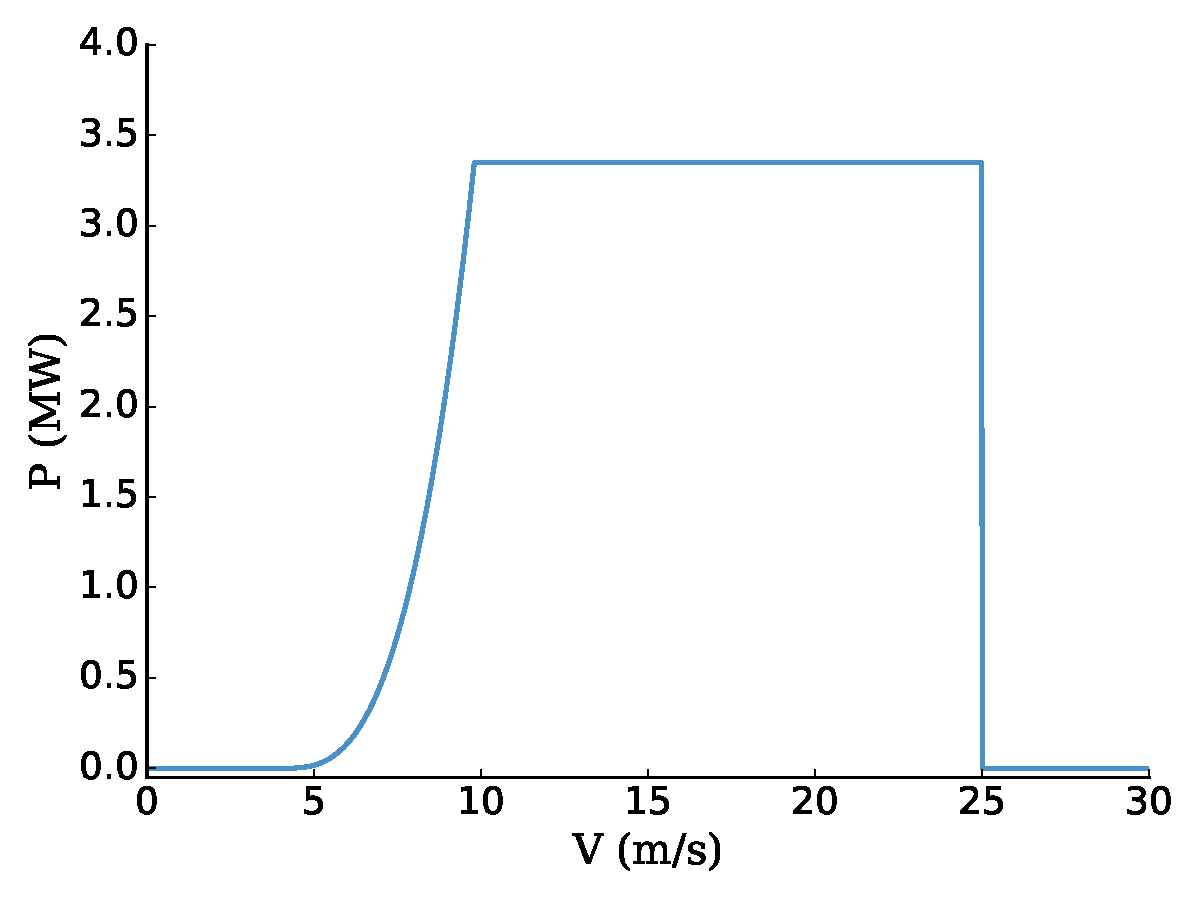
\includegraphics[width=2.6in]{./figures/iea37-335mw-pcurve.pdf}
	\end{minipage}

\subsubsection{Farm Geography}
	To focus on optimization method and EWM variability and avoid introducing too many unecessary variables, the wind farms for all scnearios are on flat and level terrain.

\vspace{3mm}
\noindent\textbf{Boundary Shape}

	\noindent As experienced by other researchers such as DUDE \cite{} and OTHER DUDE \cite{}, square and non-radially symmetric farm boundaries tend to give optimal turbine locations with turbines clustered at the farm corners or protrusions.
	For this reason, each wind farm scenario has a fixed circular boundary centered at $(0, 0)$.
	All turbine $(x, y)$ locations are constrained to remain on or within this boundary.
	In terms of spacing, no turbine can be less than two rotor diameters from any other turbine.

\vspace{3mm}
\noindent\textbf{Farm Diameter}

	\noindent Farm diameter sizing for each scenario needs to be restrictive enough to avoid simply placing all turbines on the boundary, yet also allow meaningful turbine movement by the optimizers.
	The following algorithm was implemented to determine both farm boundary diameters and the example layouts (described in the next section) for all farms in the Studies:

    \begin{enumerate}
        \item Place one turbine in the center of the farm
        \item Organize remaining turbines in concentric circles, maintaining a minimum of 5 diameter spacing
        \item If the outermost ring has less than 5 turbines:
        \begin{enumerate}
            \item Expand penultimate ring as little as possible to fit these outermost turbines, while maintaining the lateral spacing requirement
        \end{enumerate}
        \item Expand radius of outermost ring to to nearest $100$ m.
        \item Evenly expand the inner turbine rings for uniformity
    \end{enumerate}

\vspace{3mm}
\noindent\textbf{Example Layouts}

	\noindent For Case Study 1, example turbine layouts in \texttt{.yaml} format are provided, displayed graphically in \cref{fig:exlayouts}.
	These examples are supplied to participants for 4 reasons:

	\begin{enumerate}
		\item To provide an example of the \texttt{.yaml} schema desired by NREL to descirbe turbine placement
		\item To help participants visualize the different farm sizes and geography
		\item To verify AEP calculation if participants implemented the wake model in a different language
		\item To provide participants with an optimization starting point if necessary
	\end{enumerate}

	\begin{figure}[H]
		\centering
			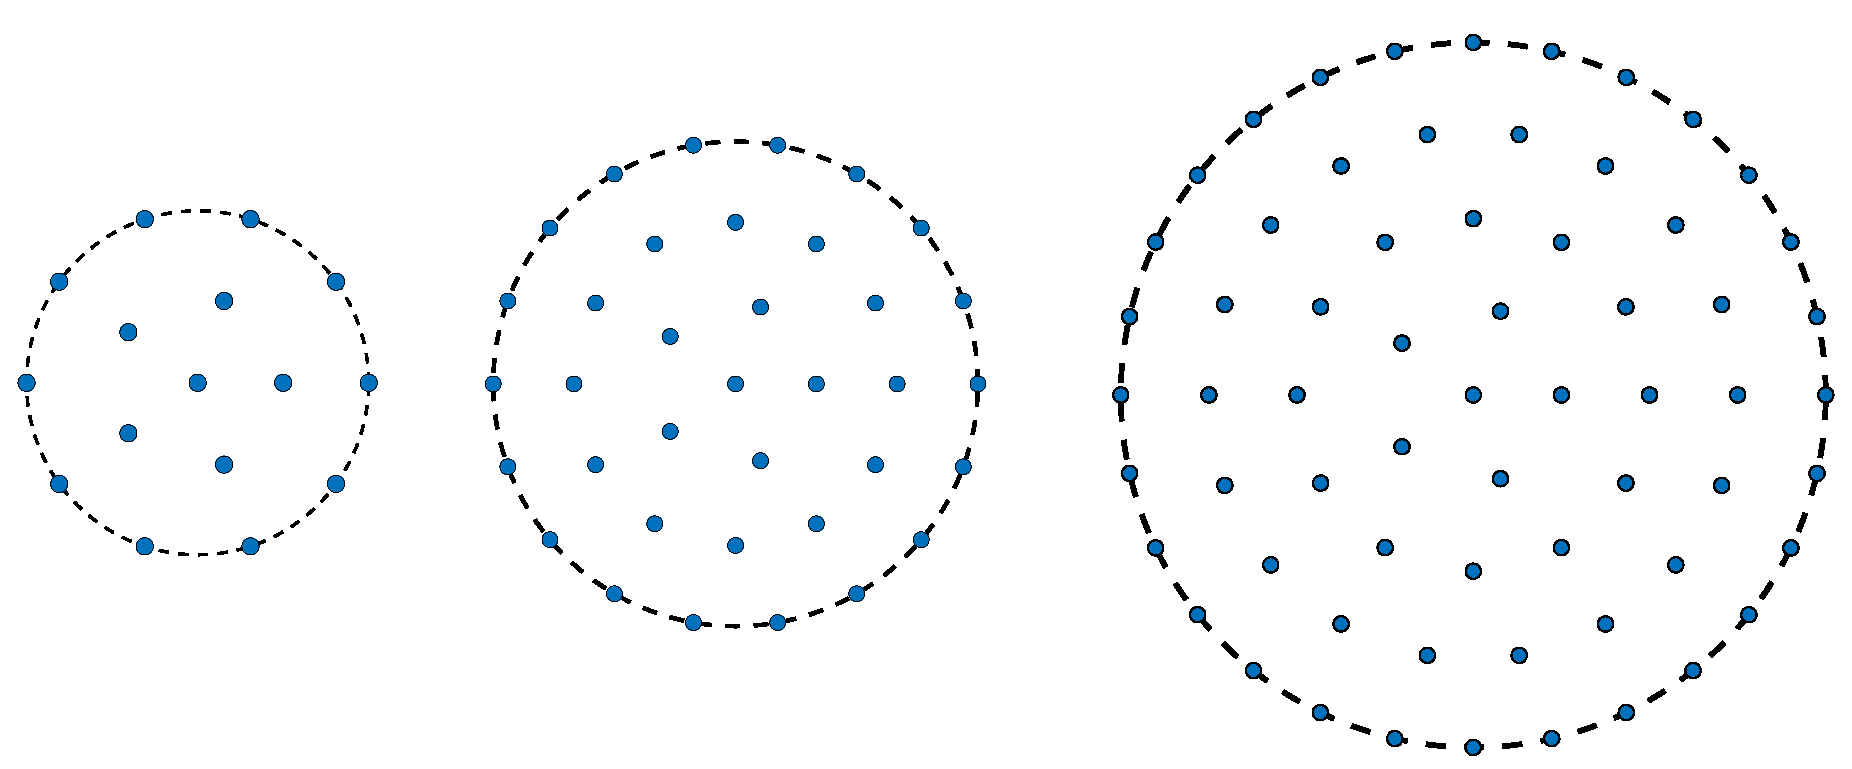
\includegraphics[width=\textwidth]{./figures/iea37-exfarms.pdf}
		\caption{Example layouts for 16, 36, and 64 turbine farms}
		\label{fig:exlayouts}
	\end{figure}

	It is explicitly stated in the announcement document that these layouts are only examples.
	Participants are not required to use these as starting points for their optimizations, though they have the option to do so.

\subsubsection{Wind Attributes}

	Again, to avoid introducing unecessary variables, the wind distribution frequency and wind speed are the same for all wind farm scenarios in both Case Studies.

\vspace{3mm}
\noindent\textbf{Wind Speed}

	\noindent Freestream wind velocity is constant throughout the farm, at $9.8\ \textrm{m/s}$, regardless of turbine location or time of day.
	$9.8\ \textrm{m/s}$ is used because it is the minimum wind speed for the NREL 3.35MW reference turbine to produce its rated power.
	Using this incoming wind velocity, turbine wakes will push air speeds down the turbine's power curve, and more local minima will be experienced by participant optimizers.
	If the incoming wind speed are too high (i.e. $13\ \textrm{m/s}$), some turbine layouts, though different in location, will produce the same power output, and avoid incentivizing optimizers to find the most efficient locations.

\vspace{3mm}
\noindent\textbf{Wind Direction Frequency}

	\noindent In creating these Case Studies, we desired a wind direction frequency (displayed graphically in a wind rose) that both creates many local minima, and permits few unique methods of reaching an optima.
	
	If there is a lack of local minima in a design space, even inefficient optimizers can find the best result.
	In a design space characterized by local minima, only the most robust optimization methods are able to escape these traps.
	For this reason, we desired a windrose that could produce many local minima.
	
	If, on the other hand, despite the presence of local minima, many non-similar layouts produce high and similar AEP values, it would likewise not tell us much regarding optimization method abilities.
	When many answers give superior results, algorithms are not incentivized to find novel or unique solutions. 
	
	Therefore to acheive both of these criteria, we experimented with 4 different patterns of wind direction frequency:

	\begin{enumerate}
		\item Bi-modal uniaxis (to simulate a canyon geography)
		\item Quad-directional (experienced at some onshore airports)
		\item Tri-direcitonal (simulating an off-shore enviornment)
		\item Bi-modal off-axis (experienced in both on- and off-shore locations)
	\end{enumerate}

	Simulations were run using the simplified Gaussian wake model and the optimization package SNOPT.
	We ran each wind rose through 1000 random-start optimizations.
	All wind roses gave generally similar results following a bell-curve pattern.
	There were slight differences, however, in that:

	\begin{enumerate}
		\item Bi-modal uniaxis gave turbine arrangements that tended towards a straight line, perpendicular to the uniaxis of the wind. Since it met our first disqualifying criteria of a lack of local minima, it was not further anilyzed.
		\item Quad-directional gave turbine arrangements that tended towards a grid pattern. Since this too didn't have many local minima to trap the optimizer, it was disqualified.
		\item Tri-directional gave many gird-like arrangements that all had similar AEP values. Since it met our second disqualifying criteria of non-similar layouts producing similar AEP, it was not selected.
		\item Bi-modal off-axis gave few results with high AEP values. We interpreted this to be indicitive of the presence of many local minima. Since this best met our selection criteria, it is the wind rose utilized for our Case Studies.
	\end{enumerate}
	
	The wind roses are binned for 16 directions. The quad-directional, tri-directional, and bi-modal off-axis roses are dipectied in \cref{fig:testroses}, and histograms of the 1000 random start optimizations are in \cref{fig:rosehists}.

	\begin{figure}[H]
		\centering
			\caption{Quad-directional, Tri-directional, and Bi-modal off-axis wind roses}
			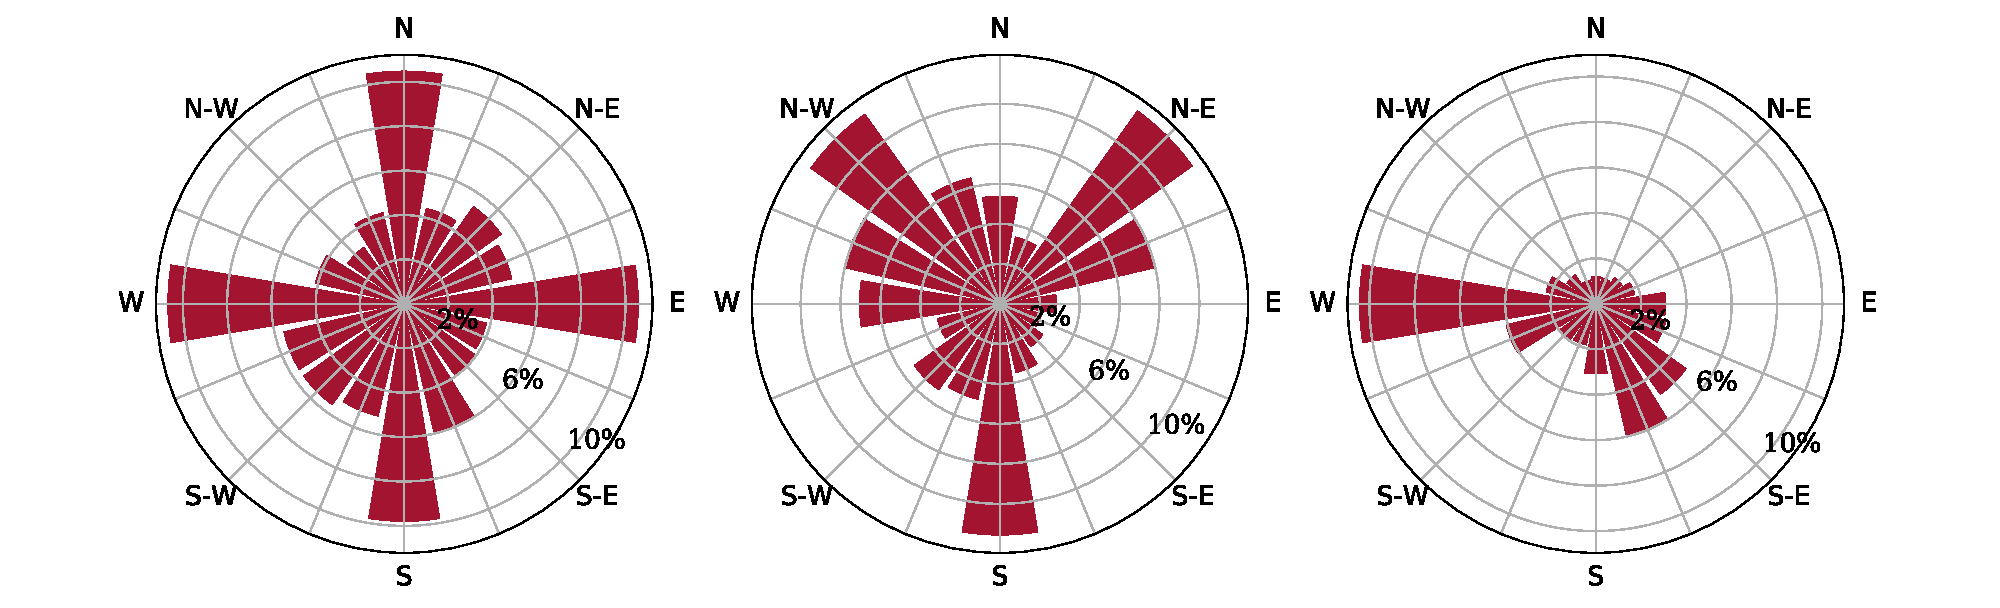
\includegraphics[width=\textwidth]{./figures/testroses.pdf}
		\label{fig:testroses}
	\end{figure}

	\begin{figure}[H]
		\centering
			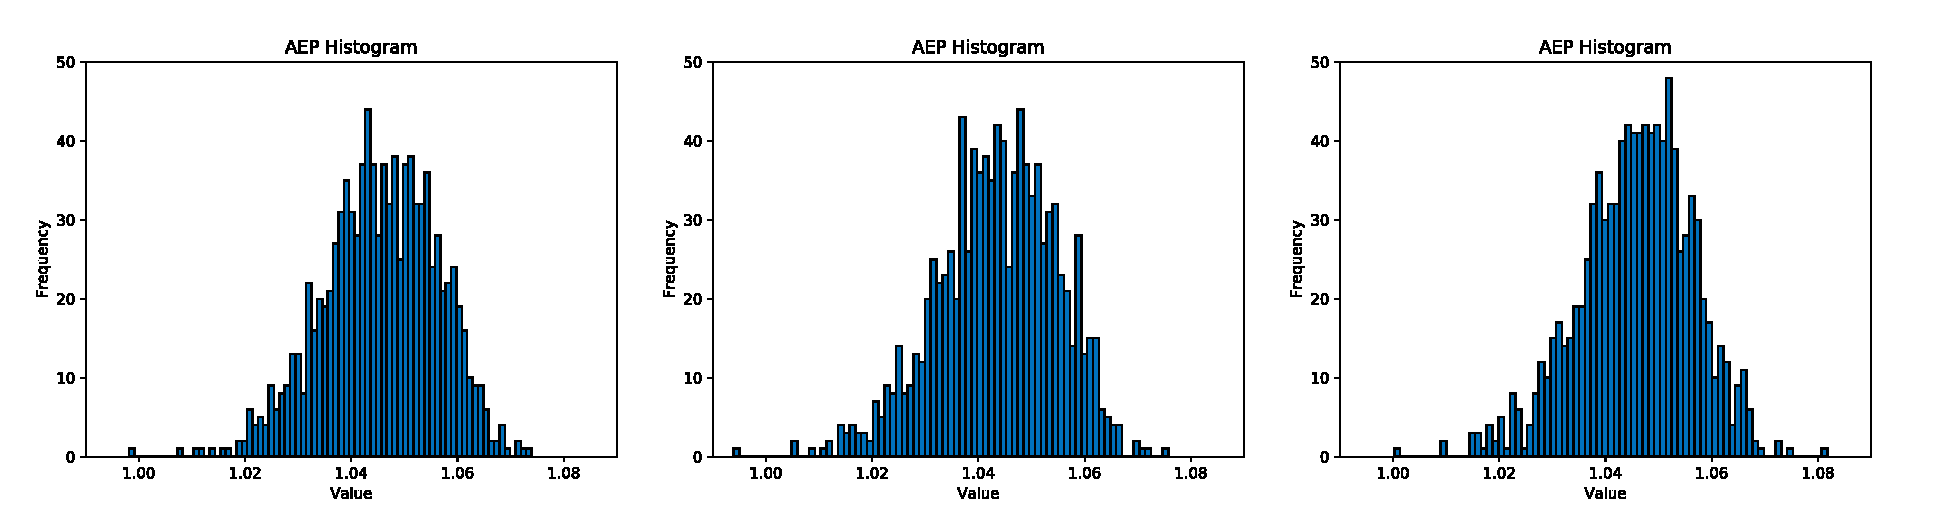
\includegraphics[width=\textwidth]{./figures/rosehists.pdf}
		\caption{1000 random start optimization runs for the Quad-, Tri-, and Bi-modal off-axis wind roses}
		\label{fig:rosehists}
	\end{figure}

	After the above described study, we selected the bi-modal off axis wind frequency distribution for our Case Studies, shown graphically below.
	A greater magnitude in the radial direction from the origin indicates a higher frequency from that cardinal direction.
	
	\begin{figure}[H]
		\centering 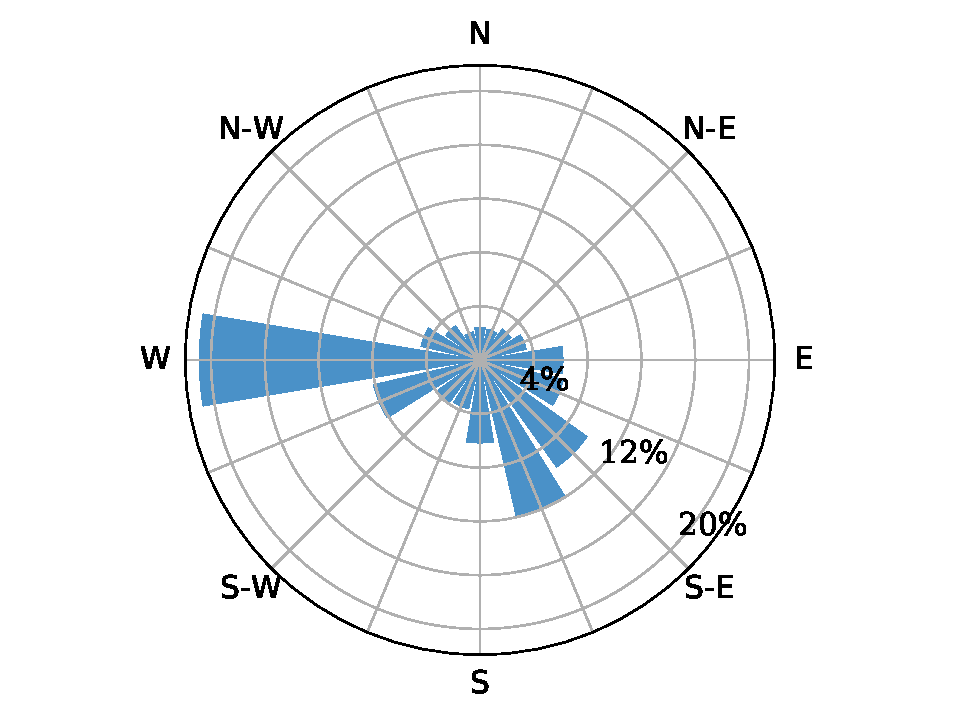
\includegraphics[width=.5\textwidth]{./figures/windrose.pdf}
		\caption{The wind frequency distribution for our Case Studies}
		\label{fig:freqdist}
	\end{figure}

\subsubsection{Data File Type} \label{sec:filetypes}
	One request made by leaders of NREL's IEA Task 37 was to implement their open source \texttt{.yaml} schema for all necessary data.
	This included:
	\begin{itemize}
		\item{Farm turbine attributes}
		\item{Farm turbine locaitons}
		\item{Farm wind frequency and wind speeds}
	\end{itemize}

	There exists a separate IEA37 working group tasked with refining the precise schema of these items, whose work is outside the scope of our specific Case Studies.
	Though a current work in progress, we implemented the most recent iteration and adapted them to our scenarios as necessary.

	The above mentioned data schema format is supplied to participants of both cases. They are:
	\begin{enumerate}
		\item \texttt{iea37-windrose.yaml} - binned wind frequency for both Case Studies, in \texttt{.yaml} format
		\item \texttt{iea37-335mw.yaml} - data for reference turbine used in both Case Studies, in \texttt{.yaml} format
	\end{enumerate}

	Further examples for reporting turbine locations in \texttt{.yaml} schema, as well as a Python parser for all these schema is available to Case Study participants.
	Since their use is more applicable to the Optimization Only Case Study, they are described in \cref{sec:optonly}.